\section{Metodología}
\subsection{Materiales y equipo}
Se utilizó un calorímetro con agitador para realizar las mezclas, un termómetro para registrar las temperaturas y una balanza para determinar las masas. Se emplearon dos vasos de precipitados de \SI{250}{\milli\liter} para preparar y medir las porciones de agua a temperatura ambiente y de agua fría. Además, se utilizó hielo, papel absorbente para retirar su humedad superficial y pinzas o cuchara para su manipulación.

\subsection{Determinación de la capacidad calorífica del calorímetro}
Se determinó la masa del vaso de precipitados vacío para descontarla de las mediciones posteriores. Las masas de las muestras de agua se midieron con una balanza mecánica, como se muestra en la Fig.~\ref{fig:balanza_calorimetria}. Se colocó en el calorímetro una porción de agua a temperatura ambiente de aproximadamente \SIrange{80}{100}{\gram} y se registraron su masa y su temperatura inicial. En el otro recipiente se preparó agua fría mediante la incorporación de hielo y se esperó hasta obtener una mezcla homogénea. De esta preparación se midió una porción de agua fría de aproximadamente \SIrange{50}{70}{\gram} y se registró su temperatura antes de efectuar la mezcla.

\begin{figure}[!htbp]
  \centering
  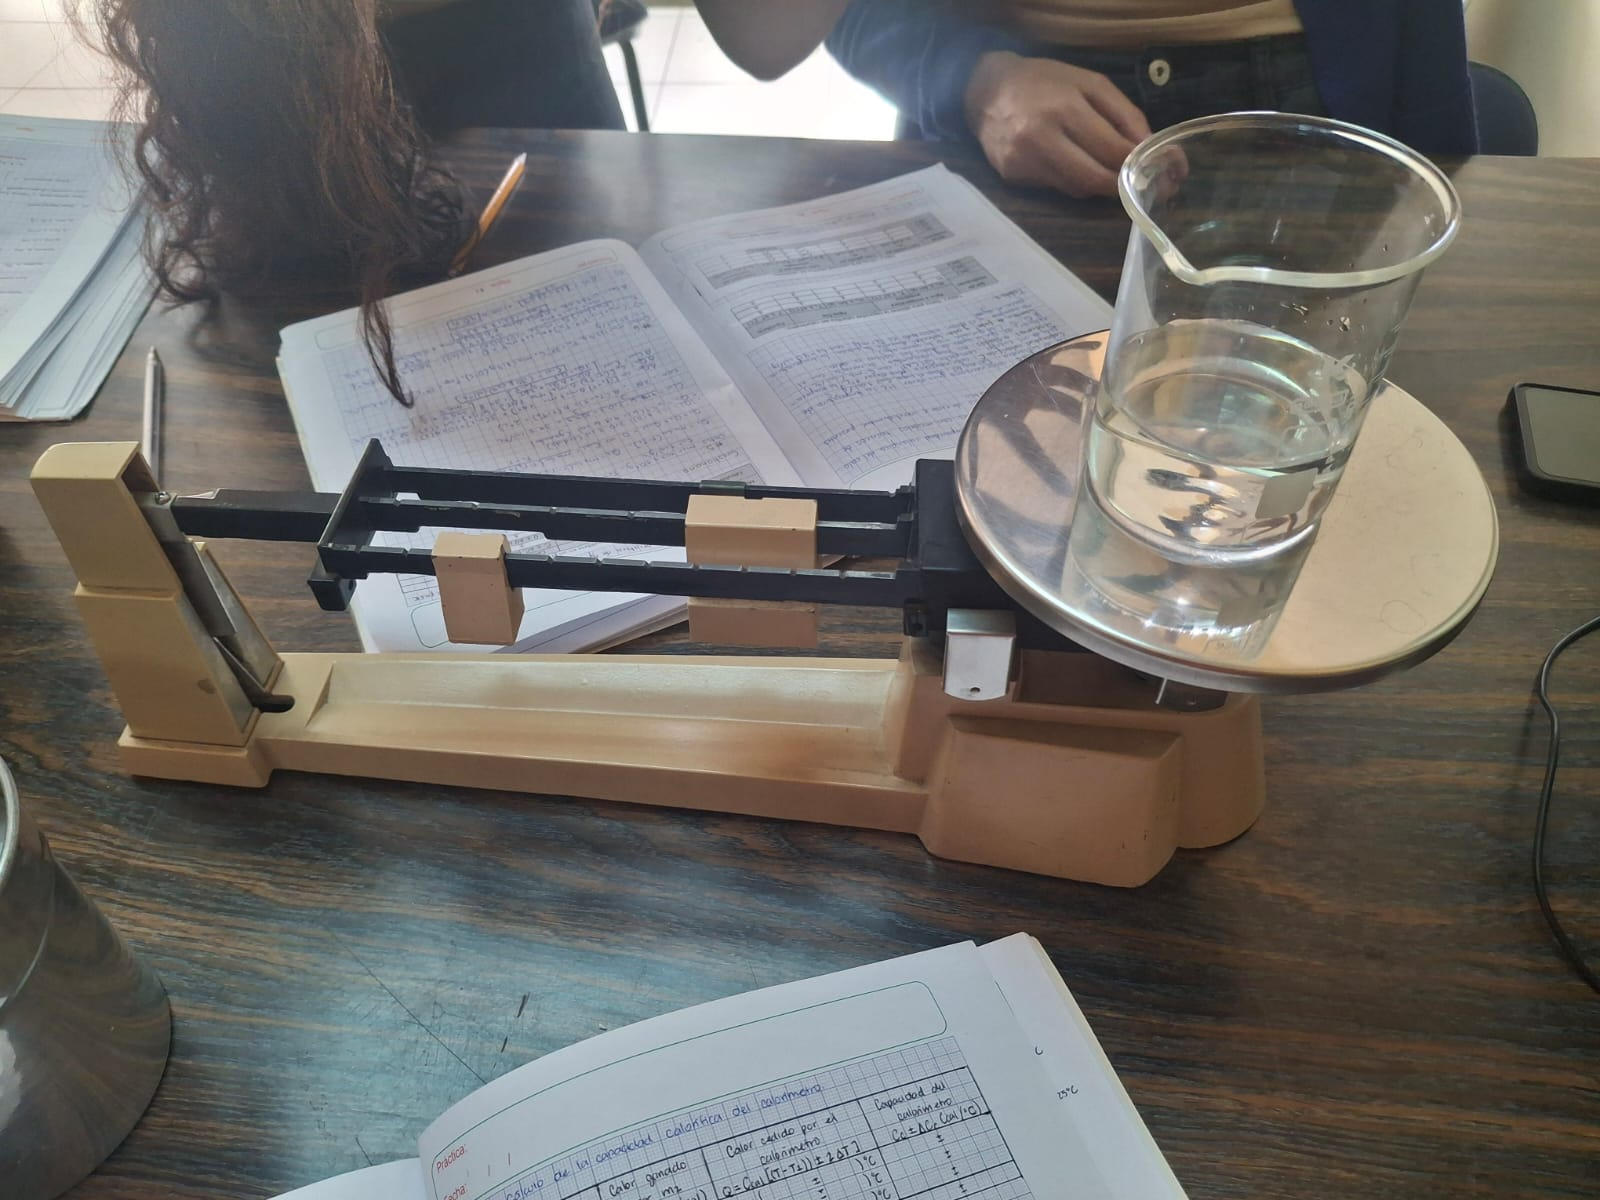
\includegraphics[width=\columnwidth,height=0.24\textheight,keepaspectratio]{figuras/balanza_calorimetria.jpeg}
  \caption{Determinación experimental de la masa del agua mediante una balanza mecánica.}
  \label{fig:balanza_calorimetria}
\end{figure}

El agua fría se incorporó rápidamente al calorímetro, que se tapó y se agitó suavemente. Se esperó hasta alcanzar el equilibrio térmico y se registró la temperatura final. El montaje empleado para registrar la temperatura de equilibrio se presenta en la Fig.~\ref{fig:montaje_calorimetro}. El procedimiento se repitió hasta obtener tres conjuntos de mediciones; entre ensayos se secó el calorímetro y se verificó nuevamente la temperatura inicial. Las masas y temperaturas registradas se emplearon para determinar la capacidad calorífica del calorímetro mediante un balance de energía entre el agua inicialmente contenida, el agua fría y el propio calorímetro.

\begin{figure}[!htbp]
  \centering
  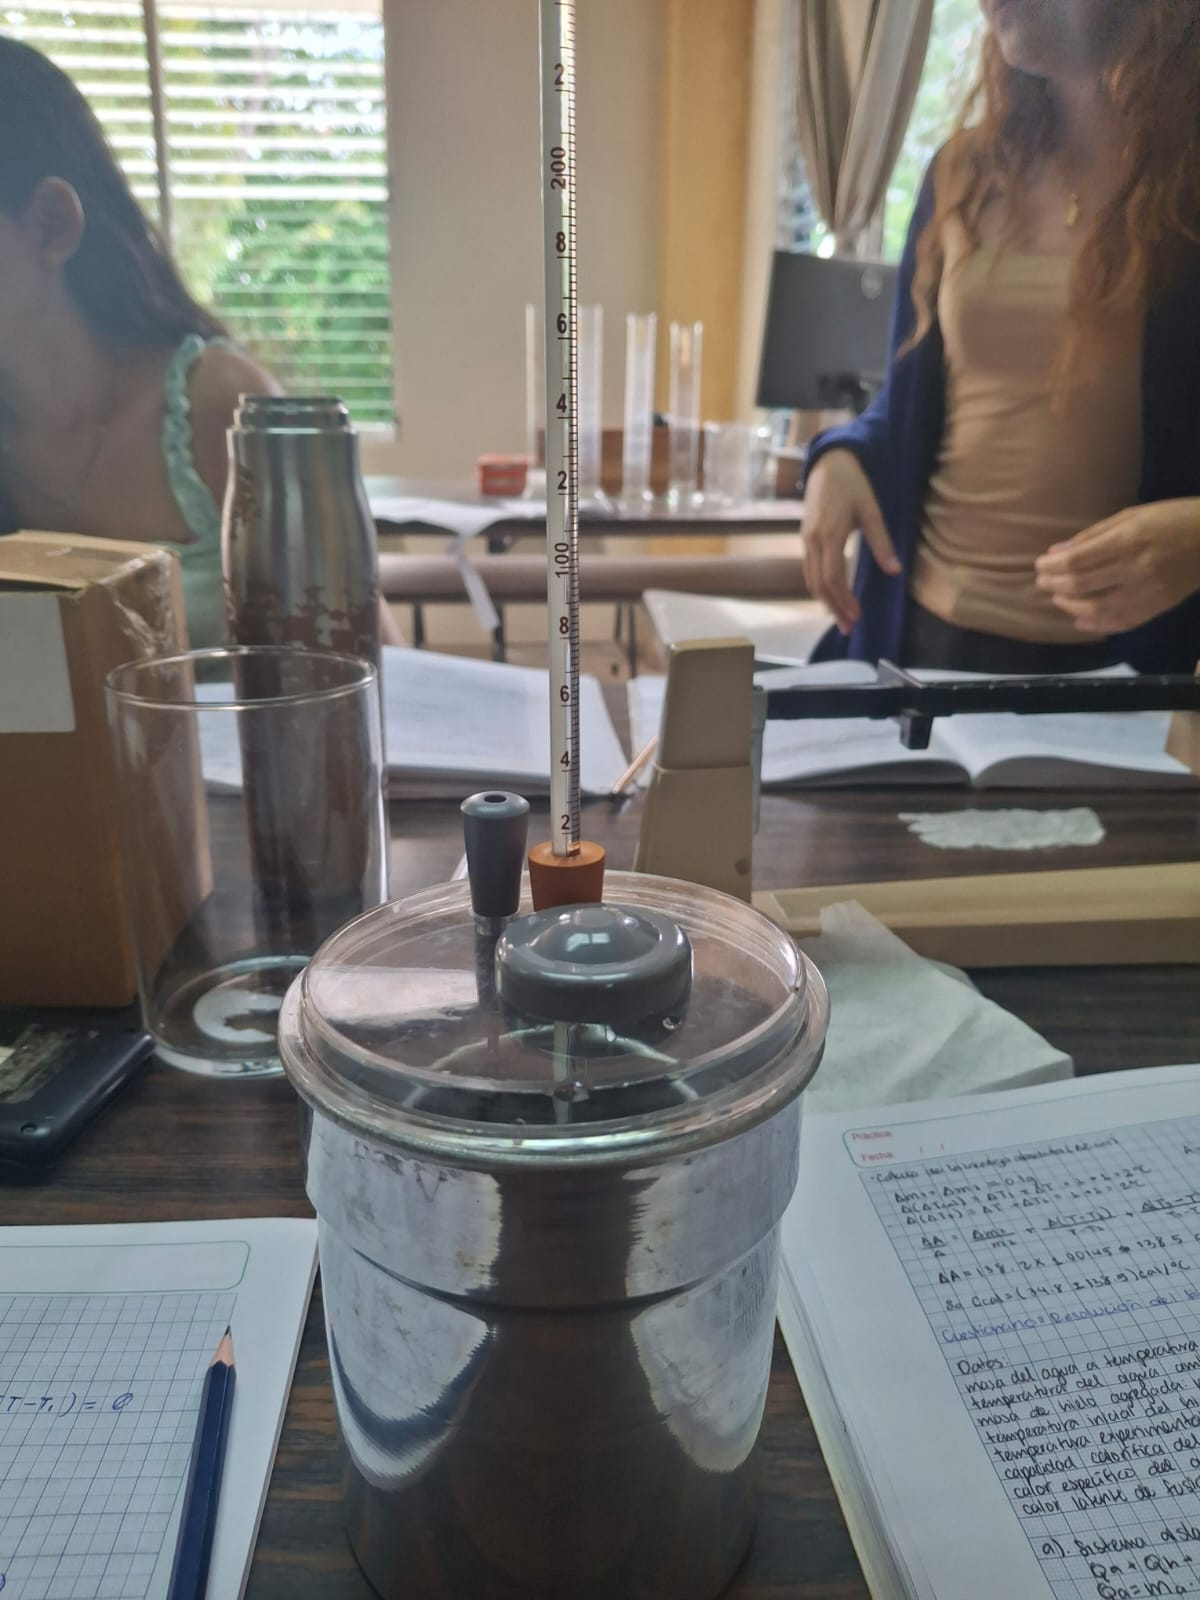
\includegraphics[width=\columnwidth,height=0.30\textheight,keepaspectratio]{figuras/montaje_calorimetro.jpeg}
  \caption{Montaje experimental del calorímetro con termómetro y sistema de agitación.}
  \label{fig:montaje_calorimetro}
\end{figure}

\subsection{Equilibrio térmico y cambio de fase}
Se colocaron aproximadamente \SIrange{120}{130}{\gram} de agua a temperatura ambiente dentro del calorímetro y se registraron su masa y su temperatura inicial. Se retiró la humedad superficial de una muestra de hielo con papel absorbente y se midió una porción de aproximadamente \SIrange{5}{15}{\gram}. El hielo se introdujo en el calorímetro utilizando pinzas; a continuación, se cerró el recipiente y se agitó suavemente hasta alcanzar el equilibrio térmico. Se registró la temperatura final experimental y se determinó la masa efectiva del hielo descontando la masa del papel absorbente de la medición correspondiente.

Se planteó un balance energético que consideró el calor cedido por el agua y el calorímetro, así como el calor absorbido durante la fusión del hielo y el calentamiento del agua resultante. A partir de este balance se calculó la temperatura teórica de equilibrio y se comparó con la temperatura experimental. También se evaluó el modelo que despreció la capacidad calorífica del calorímetro.

\subsection{Tratamiento de datos e incertidumbres}
Los datos se procesaron mediante el principio de conservación de la energía. Se utilizaron un calor específico del agua de $c_{\mathrm{agua}}=1\,\mathrm{cal}/(\mathrm{g}\cdot{}^{\circ}\mathrm{C})$ y un calor latente de fusión del hielo de $L_{\mathrm{f}}=80\,\mathrm{cal}/\mathrm{g}$. Con las masas y las variaciones de temperatura se calcularon los calores intercambiados y la capacidad calorífica del calorímetro, que se empleó en el análisis de la segunda parte.

Se consideraron las incertidumbres instrumentales de la balanza y del termómetro y su propagación en las masas obtenidas por diferencia y en las magnitudes calculadas a partir de los balances energéticos. Para ambos modelos se compararon las temperaturas teóricas y experimentales mediante el error porcentual, tomando como referencia la temperatura teórica correspondiente.
